\newpage
%%%%%%%%%%%%%%%%%%%%%%%%%%%%%%%%%%%%%%%%%%%%%%%%%%%%%%%%%%%%%%%%
%%%%%%%%%%%%%%%%%%%%%%%%%%%%%%%%%%%%%%%%%%%%%%%%%%%%%%%%%%%%%%%%
%%%%%%%%%%%%%%%%%%%%%%%%%% Enunciado %%%%%%%%%%%%%%%%%%%%%%%%%%%

\begin{myblock}
\phantomsection\addcontentsline{toc}{section}{Ejercicio \#7 | Seguros}
\section*{Ejercicio \#7 | Seguros}

Los datos dentrl del cuadro \ref{tab:seguros} son números $n$ de pólizas de seguros, y los correspondientes
numeros $y$ de reclamos (esto es, número de accidentes en los que se pidió el amparo de la poliza). La
variable \texttt{CAR} es una codificación de varias clases de carros, \texttt{EDAD} es la edad del 
titular de la póliza y \texttt{DIST} es el distrito donde vive el titular.

\textbf{(a)} Calcule la tasa de reclamos $\frac{y}{n}$ para cada categoría y grafique estas tasas contra 
las diferentes variables para tener una idea de los efectos principales. 

\end{myblock}

%%%%%%%%%%%%%%%%%%%%%%%%%%%%%%%%%%%%%%%%%%%%%%%%%%%%%%%%%%%%%%%%
%%%%%%%%%%%%%%%%%%%%%%%%%%%%%%%%%%%%%%%%%%%%%%%%%%%%%%%%%%%%%%%%

\begin{table}[h!]
    \centering
    \begin{tabular}{cc|cc|cc}
        \hline
        \textbf{CAR} & \textbf{EDAD} & \multicolumn{2}{c|}{\textbf{DIST = 0}} & \multicolumn{2}{c}{\textbf{DIST = 1}} \\
        & & \textbf{y} & \textbf{n} & \textbf{y} & \textbf{n} \\
        \hline
        1 & 1 & 65  & 317  & 2   & 20   \\
        1 & 2 & 65  & 476  & 5   & 33   \\
        1 & 3 & 52  & 486  & 4   & 40   \\
        1 & 4 & 310 & 3259 & 36  & 316  \\
        \hline
        2 & 1 & 98  & 486  & 7   & 31   \\
        2 & 2 & 159 & 1004 & 10  & 81   \\
        2 & 3 & 175 & 1355 & 22  & 122  \\
        2 & 4 & 877 & 7660 & 102 & 724  \\
        \hline
        3 & 1 & 41  & 223  & 5   & 18   \\
        3 & 2 & 117 & 539  & 7   & 39   \\
        3 & 3 & 137 & 697  & 16  & 68  \\
        3 & 4 & 477 & 3442 & 63  & 344  \\
        \hline
        4 & 1 & 11  & 40   & 0   & 3    \\
        4 & 2 & 35  & 148  & 6   & 16   \\
        4 & 3 & 39  & 214  & 8   & 25   \\
        4 & 4 & 167 & 1019 & 33  & 114  \\
        \hline
    \end{tabular}
    \caption{Numero de polizas (n) y reclamos (y) por tipo de carro, edad y distrito.}
    \label{tab:seguros}
\end{table}

%%%%%%%%%%%%%%%%%%%%%%%%%%%%%%%%%%%%%%%%%%%%%%%%%%%%%%%%%%%%%%%%
%%%%%%%%%%%%%%%%%%%%%%%%%%%%%%%%%%%%%%%%%%%%%%%%%%%%%%%%%%%%%%%%


Vamos a calcular la tasa de reclamos para cada celda de la tabla:

\[
    \text{tasa} = \frac{y}{n}
\]

Donde $y$ es el número de reclamos o accidentes reportados, y $n$ el número de pólizas. Esto nos da 
una medida de la frecuencia relativa de accidentes en cada categoría. Luego, graficaremos estas tasas 
contra las variables explicativas (\texttt{CAR}, \texttt{EDAD}, \texttt{DIST}) para visualizar los
efectos principales.  

La parte matemática formal quedaría como lo siguiente. Dado un dataset indexado por $i$ (combinaciones
de nuestras tres variables), definimos:

\[
    \hat{\pi}_i = \frac{y_i}{n_i} \;\;\;\;\; \text{con} \;\; 0 \leq \hat{pi}_i \leq 1
\]

La interpretación es que $\hat{pi}_i$ estima la probabilidad de reclamo para una póliza de la categoría $i$.

Básicamente, lo que haremos será construir nuestro dataframe en R, calcular la tasa creando una nueva
columna dentro del dataframe, a la cual podemos llamar \texttt{rate} y que esté definida por la tasa $\frac{y}{n}$.
De ese modo, graficamos cómo cambia la tasa acorde a cada variable (\texttt{CAR}, \texttt{EDAD}, \texttt{DIST}).

\subsubsection{Resultados (a)}

El gráfico de tasas específicas (Figura 1), muestra que en \texttt{DIST=0} las tasas de reclamo disminuyen
de manera consistentee a medida que aumenta la edad del titular, con diferencias clasras entre tipos de 
carro. En \texttt{DIST = 1}, el patrón es menos regular, aunque destaca un pico particularmente alto en 
\texttt{CAR=4} y \texttt{EDAD=2}, dejando entrever interacción entre variables. 

Ahora bien, podemos resumir los efectos promedio de cada variable, calculando las tasas agregadas ponderadas
por el número de pólizas, junto con intervalos de confianza binomiales. 

\begin{itemize}
    \item \textbf{CAR}: la tasa promedio aumenta de manera monótona desde \texttt{CAR=1} hasta \texttt{CAR=4}. 
    Esto indica que ciertos tipos de automóviles están asociados a mayor frecuencia de reclamos.
    \item \textbf{EDAD}: podemos notar que hay un gradiente pronnunciado negativo. Los titulares más jovenes,
    i.e. \texttt{EDAD=1} presentan tasas cercanas a 0.20, mientras que los mayores, referentes a \texttt{EDAD=4}
    alcanzan apenas 0.12. El patrón indica una disminución del riesgo de reclamo a mayor edad del titular, o conductor.
    \item \textbf{DIST}: en cuanto a los dos distritos, el distrito 1 presenta mayor tasa promedio que el 2. 
    mientras que el distrito 1 tienen 0.165 puntos, el segundo tiene 0.132. Esto puede ser un posible efecto
    de localización geográfica en el riesgo de los accidentes. 
\end{itemize}

Estos resultados no sindican que las características del automóvil, la edad del conductor y el distrito
de residencia son factores asociados de manera importante con la frecuencia de los reclamos. Las figuras
encontradas demuestran que los vehículos de categorías 3 y 4 muestran un riesgo considerablemente mayor 
a las otras. De igual forma, el riesgo de siniestros disminuye con la edad del conductor, esto hace un 
poco de sentido si tomamos en cuenta que los conductores jóvenes tienen menos experiencia al volante 
y pueden resultar un poco más temerarios al moemnto de tomar el carro. El efecto del distrito parece 
ser el de menor impacto. 

\begin{figure}[h!]
    \centering
    
    % --- Primera Fila ---
    \begin{subfigure}[b]{0.48\textwidth}
        \centering
        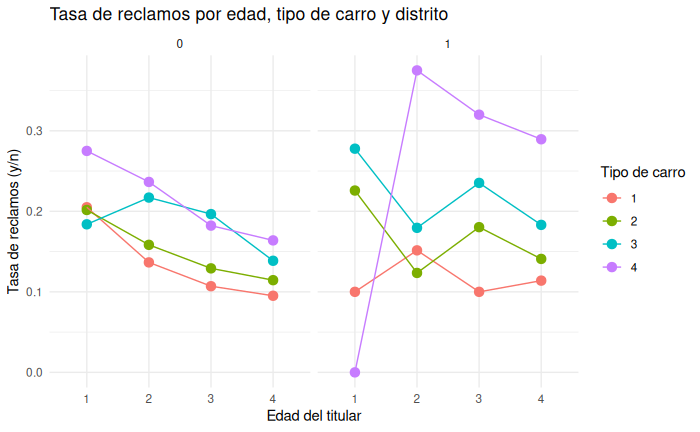
\includegraphics[width=\textwidth]{Images/tasa-reclamos-edad-titular.png}
        \caption{Tasa de las distintas variables.}
        \label{fig:img1}
    \end{subfigure}
    \hfill % Espacio horizontal entre las imágenes
    \begin{subfigure}[b]{0.48\textwidth}
        \centering
        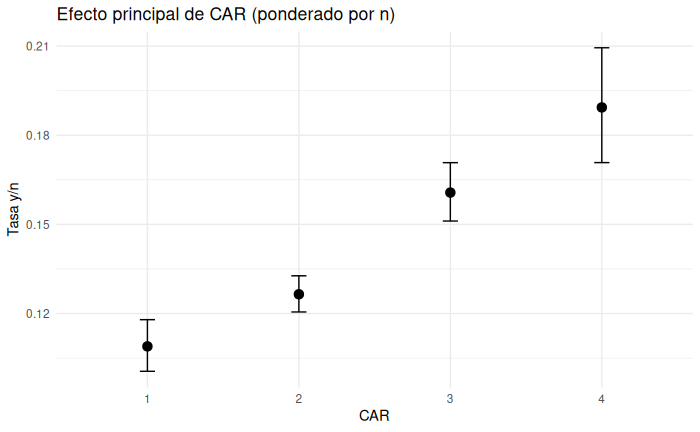
\includegraphics[width=\textwidth]{Images/CAR-seguros.png}
        \caption{Tasa vs. Carro.}
        \label{fig:img2}
    \end{subfigure}
    
    \vspace{0.5cm} % Espacio vertical entre las filas
    
    % --- Segunda Fila ---
    \begin{subfigure}[b]{0.48\textwidth}
        \centering
        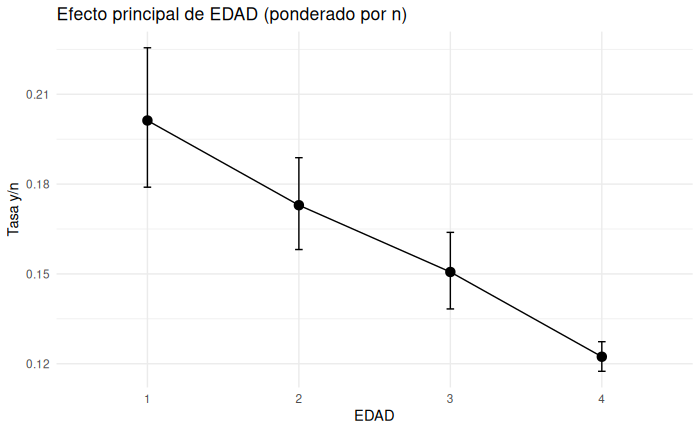
\includegraphics[width=\textwidth]{Images/EDAD-seguros.png}
        \caption{Tasa vs. Edad.}
        \label{fig:img3}
    \end{subfigure}
    \hfill % Espacio horizontal
    \begin{subfigure}[b]{0.48\textwidth}
        \centering
        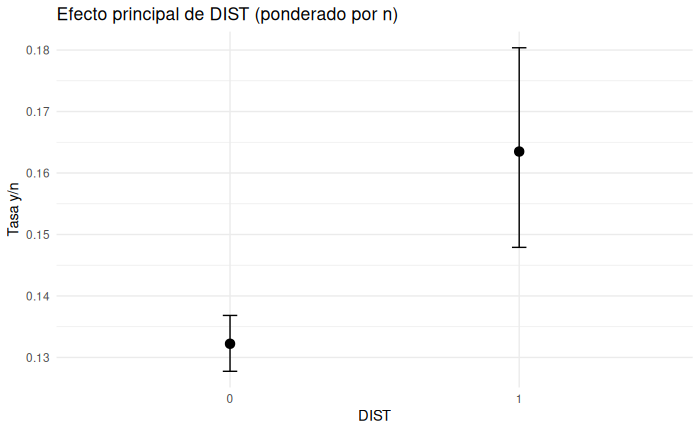
\includegraphics[width=\textwidth]{Images/DIST.png}
        \caption{Tasa vs. Distrito.}
        \label{fig:img4}
    \end{subfigure}
    
    \caption{Gráfica de las tasas vs. cada variable.}
    \label{fig:matriz_imagenes}
\end{figure}

%%%%%%%%%%%%%%%%%%%%%%%%%%%%%%%%%%%%%%%%%%%%%%%%%%%%%%%%%%%%%%%%%%%%%%%%%%%%%
%%%%%%%%%%%%%%%%%%%%%%%%%%%%%%%%%%%%%%%%%%%%%%%%%%%%%%%%%%%%%%%%%%%%%%%%%%%%%

\begin{myblock}
    
    \textbf{(b)} Ajusta un modelo de Poisson apropiado. 

\end{myblock}

\subsubsection{Modelo GLM Poisson}

Ajustamos un modelo GLM Poisson para los conteos $y_i$ con enlace log y \text{offset} $log(n_i)$:

\[
    y_i \sim Poisson(y_i) \;\;\;\;\; log(y_i) = log(n_i) + \beta_0 + \beta(\text{CAR}) + \beta(\text{EDAD}) + \beta(\text{DIST})
\]

De los tres modelos $(m_0 = 378.19, m_1 = 208.07, m_2 = 219.66)$, el modelo $m_1$ es el que tiene el AIC mínimo. 
La Binomial Negativa no mejora, por lo que el modelo final es Poisson con una combinación de las variables. 

\begin{table}[h!]
    \centering
    \caption{Resumen de IRR (Incidence Rate Ratios) del modelo final.}
    \label{tab:irr_summary}
    \begin{tabular}{l l c c l p{6cm}}
        \toprule
        \textbf{Variable} & \textbf{Nivel} & \textbf{IRR} & \textbf{IC al 95\%} & \textbf{Valor p} & \textbf{Interpretación} \\
        \midrule
        
        \multicolumn{6}{l}{\textit{Tipo de carro (CAR)}} \\
        & CAR=4 & 1.76 & $[1.53 - 2.03]$ & $< 10^{-14}$ & A exposición fija, presenta una tasa 76\% mayor que CAR=1. Efecto grande y muy preciso. \\
        & CAR=3 & 1.48 & $[1.33 - 1.65]$ & $< 10^{-12}$ & Tasa 48\% mayor que CAR=1; también alto y preciso. \\
        & CAR=2 & 1.18 & $[1.07 - 1.30]$ & $0.0013$ & Incremento moderado ($\approx 18\%$) pero estadísticamente significativo. \\
        \midrule

        \multicolumn{6}{l}{\textit{Edad del titular (EDAD)}} \\
        & EDAD=4 & 0.587 & $[0.512 - 0.673]$ & $< 10^{-13}$ & 41\% menor tasa respecto a EDAD=1; efecto fuerte y preciso. \\
        & EDAD=3 & 0.710 & $[0.606 - 0.833]$ & $2.6 \times 10^{-5}$ & 29\% menor. \\
        & EDAD=2 & 0.828 & $[0.704 - 0.974]$ & $0.022$ & 17\% menor (efecto pequeño a moderado). \\
        \midrule

        \multicolumn{6}{l}{\textit{Distrito (DIST)}} \\
        & DIST=1 & 1.244 & $[1.109 - 1.395]$ & $1.9 \times 10^{-4}$ & Tasa 24\% mayor que DIST=0; efecto moderado y bien estimado. \\
        \midrule

        \multicolumn{6}{l}{\textit{Intercepto}} \\
        & Tasa base & 0.164 & $[0.141 - 0.190]$ & - & Tasa base para la categoría de referencia (CAR=1, EDAD=1, DIST=0). \\
        \bottomrule
    \end{tabular}
\end{table}


\begin{figure}[h!]
    \centering
    % --- Imagen Superior ---
    \begin{subfigure}[b]{0.8\textwidth} % Ancho de la subfigura
        \centering
        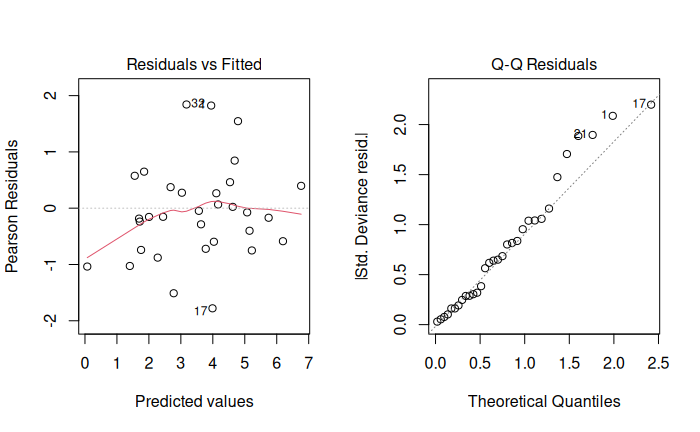
\includegraphics[width=\textwidth]{Images/modelo-poisson-seguros.png}
        \caption{Diagnóstico de residuos (m1).}
        \label{fig:img_top}
    \end{subfigure}
    
    \vspace{0.5cm} % Espacio vertical entre las imágenes
    
    % --- Imagen Inferior ---
    \begin{subfigure}[b]{0.8\textwidth} % Ancho de la subfigura
        \centering
        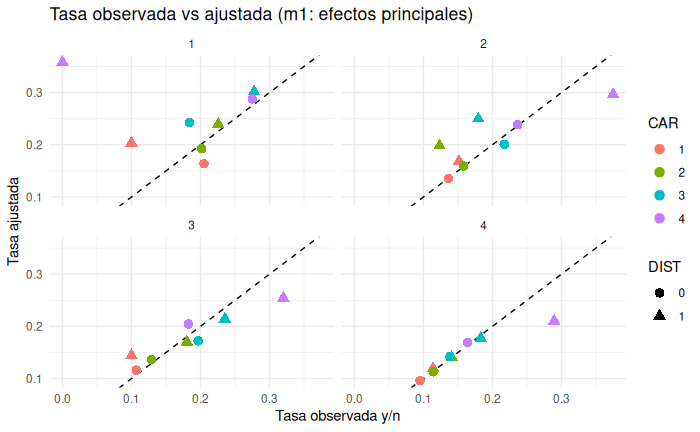
\includegraphics[width=\textwidth]{Images/tasa-obs-vs-ajustada-poisson-seguros.png}
        \caption{Tasa observada vs. ajustada (m1).}
        \label{fig:img_bottom}
    \end{subfigure}
    
    \caption{Resultados del GLM Poisson.}
    \label{fig:matriz_vertical}
\end{figure}




%%%%%%%%%%%%%%%%%%%%%%%%%%%%%%%%%%%%%%%%%%%%%%%%%%%%%%%%%%%%%%%%%%%%%%%%%%%%%
%%%%%%%%%%%%%%%%%%%%%%%%%%%%%%%%%%%%%%%%%%%%%%%%%%%%%%%%%%%%%%%%%%%%%%%%%%%%%

\begin{myblock}
    
    \textbf{(c)} Usando la normalidad asintótica de los estimadores de máxima verosimlitud, da un 
     intervalo del 90\% de confianza para la diferencia en medias. Hay evidencia de diferencias en los
     dos grupos en cuanto a las medias de los conteos?
\end{myblock}

Sea $y_g \sim \text{Poisson}(n_g\lambda_g)$ para $g \in \{0,1\}$ (distritos), con $n_g$ pólizas (exposición) y $\lambda_g$ la tasa por póliza.

El EMV es $\hat{\lambda}_g = y_g/n_g$ y, asintóticamente,
\[
    \operatorname{Var}(\hat{\lambda}_g) \approx \frac{\lambda_g}{n_g} \quad \Rightarrow \quad \widehat{\operatorname{Var}}(\hat{\lambda}_g) \approx \frac{\hat{\lambda}_g}{n_g}.
\]
Para la diferencia de medias $\Delta = \lambda_1 - \lambda_0$,
\[
    \hat{\Delta} = \hat{\lambda}_1 - \hat{\lambda}_0, \qquad \widehat{\operatorname{SE}}(\hat{\Delta}) = \sqrt{\frac{\hat{\lambda}_1}{n_1} + \frac{\hat{\lambda}_0}{n_0}}.
\]
Un IC del 90\% (normal) es
\[
    \hat{\Delta} \pm z_{0.95}\,\widehat{\operatorname{SE}}(\hat{\Delta}), \qquad z_{0.95} = 1.6449.
\]

Sumando por distrito (de la tabla original):
\[
    y_0=2825, \; n_0=21365 \quad \Rightarrow \quad \hat{\lambda}_0=0.13223.
\]
\[
    y_1=326, \; n_1=1994 \quad \Rightarrow \quad \hat{\lambda}_1=0.16349.
\]

Diferencia:
\[
    \hat{\Delta} = 0.16349 - 0.13223 = 0.03126.
\]

Error estándar:
\[
    \widehat{\operatorname{SE}} = \sqrt{\frac{0.16349}{1994} + \frac{0.13223}{21365}} = 0.00939.
\]

IC 90\%:
\[
    0.03126 \pm 1.6449 \times 0.00939 = (0.01582, \; 0.04671).
\]

Por lo tanto, en promedio, \texttt{DIST=1} tiene entre 1.6 y 4.7 reclamos adicionales por cada 100 pólizas,
respecto a \texttt{DIST=0}. El intervalo no incluye a 0, por lo que hay evidencia de que existe diferencia
en las medias de los conteos entre distritos al 90\%. Esto, a su vez, es coherente con lo encontrado
por el IRR > 1 del inciso anterior. 



%%%%%%%%%%%%%%%%%%%%%%%%%%%%%%%%%%%%%%%%%%%%%%%%%%%%%%%%%%%%%%%%%%%%%%%%%%%%%
%%%%%%%%%%%%%%%%%%%%%%%%%%%%%%%%%%%%%%%%%%%%%%%%%%%%%%%%%%%%%%%%%%%%%%%%%%%%%




%%%%%%%%%%%%%%%%%%%%%%%%%%%%%%%%%%%%%%%%%%%%%%%%%%%%%%%%%%%%%%%%%%%%%%%%%%%%%
%%%%%%%%%%%%%%%%%%%%%%%%%%%%%%%%%%%%%%%%%%%%%%%%%%%%%%%%%%%%%%%%%%%%%%%%%%%%%






%\subsection{Teoría}

%\subsection{Resumen de código}

%\subsection{Resultados}

%\subsection{Conclusiones}

\clearpage